%%
%% MASCOTS 2026 submission.
%% IEEE conference format. IEEEtran.cls is bundled in this folder.
%%
%% Build:
%%   pdflatex paper && pdflatex paper   (run twice for cross-references)
%%   figures/fig_bootstrap.pdf and figures/fig_per_cluster.pdf are
%%   produced by:  python make_figures.py
%%
\documentclass[conference]{IEEEtran}

% --- Packages ---------------------------------------------------------------
\usepackage{amsmath,amssymb}
\usepackage{graphicx}
\usepackage{booktabs}
\usepackage{array}
\usepackage{cite}
\usepackage{xcolor}
\usepackage[hyphens]{url}
\usepackage[hidelinks]{hyperref}
\usepackage{tikz}
\usetikzlibrary{positioning,arrows.meta,fit,backgrounds,calc}

\providecommand{\SECt}{\mathrm{SEC}}

% --- TikZ block styles ------------------------------------------------------
\tikzset{
  blk/.style={draw,rounded corners=1.5pt,align=center,inner sep=2.6pt,
              font=\scriptsize,minimum height=7mm,fill=gray!6},
  grp/.style={draw,rounded corners=2.5pt,inner sep=4.5pt,line width=0.5pt},
  fl/.style={-{Latex[length=1.4mm]},line width=0.5pt},
}

\begin{document}

% ---------------------------------------------------------------------------
\title{A Measurement-Grounded Digital Twin for Evaluating Cooperative
MARL in Energy-Aware 5G UPF Orchestration}

\author{%
\IEEEauthorblockN{Shima Afshar Borji\IEEEauthorrefmark{1},
Roberto Bruschi\IEEEauthorrefmark{1}\IEEEauthorrefmark{2},
Chiara Lombardo\IEEEauthorrefmark{1}\IEEEauthorrefmark{2},
Raffaele Bolla\IEEEauthorrefmark{1}\IEEEauthorrefmark{2},
Cristina Emilia Costa\IEEEauthorrefmark{2}}
\IEEEauthorblockA{\IEEEauthorrefmark{1}DITEN, University of Genoa, Genoa, Italy \qquad
\IEEEauthorrefmark{2}CNIT -- S2N National Lab, Genoa, Italy\\
\texttt{\footnotesize shima.afshar.borji@edu.unige.it}\\
\texttt{\footnotesize \{roberto.bruschi,\,chiara.lombardo,\,raffaele.bolla\}@unige.it,\;ccosta@cnit.it}}
}

\maketitle

% ---------------------------------------------------------------------------
\begin{abstract}
The 5G User Plane Function (UPF) can run as a DPDK kernel-bypass stack,
which offers high throughput at a high idle-power floor, or as a
user-space (USR) stack, which draws less power but has a narrower safe
operating envelope. Selecting the right realization per site, across a
fleet of heterogeneous Mobile Edge Computing (MEC) clusters, is a
cooperative control problem whose multi-site coordination structure has
not been studied. We build a measurement-grounded digital twin
calibrated on a physical testbed through RAPL power measurements and
per-mode surrogate models, and use it to evaluate cooperative
multi-agent reinforcement learning (MARL) for joint UPF realization
switching across $K\,{=}\,10$ clusters. MAPPO, with a shared-parameter
actor and a centralised critic, outperforms an independent per-site PPO
(IPPO) ensemble, a centralised single-MLP PPO, and the swept-best
classical hysteresis baseline by 10 to 61\% under a physics-grounded
reward that folds measured switching energy into specific energy
consumption. The win over IPPO is small in magnitude but statistically
robust (paired bootstrap one-sided $p\,{=}\,0.009$, 95\% CI
$[+28,+262]$ reward units), and it concentrates on the data-poor
low-load clusters where independent learning lacks cross-site signal.
The result indicates that coordination architecture matters more than
algorithm choice for energy-aware UPF orchestration at the edge.
\end{abstract}

\begin{IEEEkeywords}
5G User Plane Function, energy efficiency, cooperative multi-agent
reinforcement learning, MAPPO, digital twin, mobile edge computing, CTDE.
\end{IEEEkeywords}

% ===========================================================================
\section{Introduction}
% ===========================================================================
\IEEEPARstart{T}{he} proliferation of 5G base stations and core network
functions is driving a sharp increase in telecommunications energy
consumption. The User Plane Function (UPF), which is responsible for
packet routing, forwarding, and QoS enforcement in the 5G Core, is the
highest-throughput data-plane element in a typical mobile operator
deployment and one of its largest energy consumers at the network
edge~\cite{ref:carbon}. Operators face growing pressure to reduce their
carbon footprint while maintaining stringent QoS commitments across a
geographically distributed fleet of MEC clusters.

Two UPF realization classes define the practical energy-performance
design space. A DPDK-accelerated kernel-bypass stack delivers high
throughput and low tail latency, at the cost of dedicated CPU cores held
at an elevated idle-power floor regardless of the offered load. A
user-space (USR) software stack draws substantially less power at low
utilization, but it has a narrower safe operating envelope before delay
and packet loss degrade below QoS targets~\cite{ref:rischke}. Static
all-DPDK provisioning, which is the current industry default, wastes
energy whenever traffic falls below the per-site break-even point, while
static all-USR violates QoS during peaks. The question is when to run
which realization, on a per-site basis, given noisy short-horizon
traffic forecasts and non-negligible switching costs.

Hysteresis-based switching provides the strongest classical answer.
Upper and lower thresholds derived from the energy-performance crossover
point gate transitions and prevent rapid oscillation near the decision
boundary. At a single site this approach achieves meaningful energy
savings~\cite{ref:slices}, yet it faces a fundamental limit at practical
forecaster accuracy levels. The hysteresis band must scale with the
forecaster mean absolute error (MAE) to filter noise reliably, but when
the MAE is large relative to the decision threshold, the lower threshold
collapses to zero and the controller never leaves DPDK regardless of
actual load. Single-site reinforcement learning (RL) resolves this by
learning a policy that handles forecast uncertainty
directly~\cite{ref:comcom}, but when each of $K$ heterogeneous MEC
clusters trains independently, data-poor low-load sites lack sufficient
sample signal to discover that USR is safe at their operating point.
Independent per-site learning leaves each cluster's policy bounded by its
own experience, with no mechanism to transfer the ``USR-at-low-load''
rule learned on data-rich clusters to the low-traffic sites that need it
most.

The natural remedy is cooperative multi-agent training. A
shared-parameter actor trained simultaneously across all clusters can
propagate policies across sites, while decentralised execution preserves
per-site autonomy at inference time. Whether this coordination benefit
materialises in practice, and whether it is statistically significant
relative to independent per-site learning, has not been quantified for
UPF orchestration. Answering this question requires a simulation
environment whose fidelity to real hardware is established by
measurement, so that results are grounded in actual energy-performance
trade-offs rather than synthetic assumptions.

This paper makes three contributions.
\begin{itemize}
\item \emph{A measurement-grounded digital twin for multi-site UPF
evaluation.} We calibrate a digital twin on a physical testbed (Keysight
LoadCore traffic generation, RAPL-via-Scaphandre power measurement,
SD-Core DPDK UPF and OAI USR UPF) and extend the single-site framework
of~\cite{ref:comcom} to $K\,{=}\,10$ heterogeneous MEC clusters with
distinct traffic profiles and per-mode MLP surrogate models for power
and QoS.
\item \emph{A physics-grounded reward that unifies switching and
steady-state energy.} We remove the redundant flat switching-cost
constant of prior formulations~\cite{ref:comcom} and fold the measured
activation spike energy directly into the specific energy consumption
(SEC) term, so switching costs emerge from testbed-measured activation
durations rather than hand-set constants.
\item \emph{Evidence that coordination architecture matters more than
algorithm.} A controlled three-architecture comparison at eight training
seeds, between MAPPO with a shared-parameter actor and centralised
critic~\cite{ref:mappo}, an IPPO ensemble~\cite{ref:sb3}, and a
centralised single-MLP PPO, shows that the MAPPO architectural win over
IPPO is significant at $p\,{=}\,0.009$ (paired bootstrap, 95\% CI
$[+28,+262]$ reward units), with the gain concentrating on low-load
clusters where independent learning lacks sufficient signal.
\end{itemize}

The remainder of the paper is organised as follows.
Section~\ref{sec:related} reviews related work.
Section~\ref{sec:model} describes the system model and digital twin.
Section~\ref{sec:problem} formalises the multi-site control problem and
reward. Section~\ref{sec:method} details the MARL architectures and the
evaluation protocol. Section~\ref{sec:results} presents and analyses
results, and Section~\ref{sec:conclusion} concludes.

% ===========================================================================
\section{Related Work}
\label{sec:related}
% ===========================================================================
\noindent\textbf{Rule-based UPF realization selection.}
Among classical strategies for dynamic network function management,
hysteresis-based switching is the strongest and most practically
deployable. A hysteresis policy defines an upper threshold $t_{up}$ and a
lower threshold $t_{down}\,{=}\,t_{up}\,{-}\,b$ around the
energy-performance crossover point. A switch to the low-power realization
is triggered only when predicted traffic falls below $t_{down}$, and a
switch back occurs only above $t_{up}$. The band $b$ acts as a noise
filter that prevents rapid oscillation around the decision boundary.
Simpler threshold policies, which switch on a single crossing without
hysteresis, are strictly inferior, since they are susceptible to every
forecaster error and incur excessive switching cost. This makes
hysteresis the correct classical baseline rather than the bare threshold.
Our prior work~\cite{ref:slices} studies this approach at a single site
using polynomial surrogate models and an LSTM forecaster, achieving
10.46\% energy savings over static DPDK provisioning. However,
hysteresis faces a fundamental trade-off at real forecaster accuracy
levels. The band $b$ must be set proportionally to the forecaster MAE to
filter noise reliably, yet this same scaling causes $t_{down}$ to
collapse towards zero when the MAE is large relative to the decision
threshold, at which point the controller never leaves DPDK regardless of
the actual load. We derive both thresholds directly from our calibrated
digital twin and sweep the band over five values to identify the
strongest classical operating point, so that the comparison is fair and
not based on hand-tuned parameters (Section~\ref{sec:results}). UPF
placement and chaining across the network have been studied from an
optimisation perspective~\cite{ref:leyva}, but the per-site
realization-selection problem with heterogeneous energy-performance
profiles and practical forecaster noise has received less attention.

\noindent\textbf{Reinforcement learning for single-site UPF
orchestration.} RL has been applied to UPF realization selection at a
single site. Bellin et al.~\cite{ref:bellin} use deep RL to choose among
UPF deployment options based on power consumption at the 5G edge. Our
prior work~\cite{ref:comcom} formulates the DPDK/USR selection problem as
a single-site Markov decision process trained on a measurement-grounded
digital twin, achieving 16.9\% energy savings over static DPDK
provisioning with a physics-grounded reward. These single-agent
formulations leave the multi-site coordination problem open, because each
site learns independently and data-poor low-load clusters receive no
benefit from the richer experience of high-load peers. The present paper
extends the twin-based framework to $K\,{=}\,10$ heterogeneous clusters
and directly quantifies how much coordination across sites is worth.

\noindent\textbf{Multi-agent RL for network resource management.}
Cooperative MARL has been applied to network slicing, resource
allocation, and traffic steering in MEC environments~\cite{ref:zhu}.
Value-decomposition methods such as QMIX~\cite{ref:qmix} and
VDN~\cite{ref:vdn} impose a monotonic factorisation of the joint value
function, which simplifies credit assignment but introduces an inductive
bias poorly suited to the heterogeneous reward scales of our $K\,{=}\,10$
deployment. Moreover, both are off-policy and require replay buffers,
which add tuning complexity that conflicts with the episodic,
short-horizon structure of the 15-minute UPF control problem. On-policy
actor-critic methods, specifically the MAPPO architecture~\cite{ref:mappo}
with a shared-parameter actor and a centralised critic, provide
Centralised Training with Decentralised Execution (CTDE) without these
constraints and have shown competitive performance in cooperative
discrete-action tasks. We adopt MAPPO as our proposed architecture and
include an IPPO ensemble~\cite{ref:sb3} and a centralised single-MLP PPO
as the two natural ablation points.

\noindent\textbf{Digital twins for network control evaluation.}
Measurement-grounded digital twins have emerged as a principled approach
to training and evaluating network controllers without incurring the cost
and risk of live closed-loop experimentation~\cite{ref:ndt,ref:comcom}.
The fidelity of the twin is critical, since a surrogate that does not
capture the energy-performance trade-offs of the underlying hardware will
produce controllers that misfire at deployment. We address this by
calibrating the twin on per-mode profiling data from a physical testbed
and grounding activation durations and power curves in RAPL
measurements~\cite{ref:rapl}, extending the single-site calibration
of~\cite{ref:comcom} to a ten-cluster heterogeneous fleet.

% --- Figure 1: pipeline -----------------------------------------------------
\begin{figure}[!t]
\centering
\resizebox{\columnwidth}{!}{%
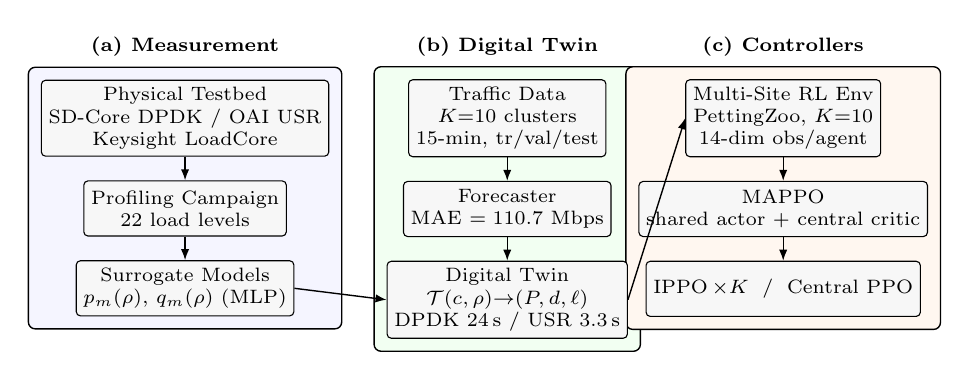
\begin{tikzpicture}[node distance=3mm]
% stage a
\node[blk] (test)  {Physical Testbed\\\scriptsize SD-Core DPDK / OAI USR\\\scriptsize Keysight LoadCore};
\node[blk,below=of test] (prof) {Profiling Campaign\\\scriptsize 22 load levels};
\node[blk,below=of prof] (surr) {Surrogate Models\\\scriptsize $p_m(\rho),\,q_m(\rho)$ (MLP)};
\begin{scope}[on background layer]
\node[grp,fill=blue!4,fit=(test)(prof)(surr),label={[font=\scriptsize\bfseries]above:(a) Measurement}] (ga) {};
\end{scope}
% stage b
\node[blk,right=10mm of test] (traf) {Traffic Data\\\scriptsize $K{=}10$ clusters\\\scriptsize 15-min, tr/val/test};
\node[blk,below=of traf] (fore) {Forecaster\\\scriptsize MAE $=110.7$ Mbps};
\node[blk,below=of fore] (twin) {Digital Twin\\\scriptsize $\mathcal{T}(c,\rho){\to}(P,d,\ell)$\\\scriptsize DPDK 24\,s / USR 3.3\,s};
\begin{scope}[on background layer]
\node[grp,fill=green!5,fit=(traf)(fore)(twin),label={[font=\scriptsize\bfseries]above:(b) Digital Twin}] (gb) {};
\end{scope}
% stage c
\node[blk,right=10mm of traf] (env) {Multi-Site RL Env\\\scriptsize PettingZoo, $K{=}10$\\\scriptsize 14-dim obs/agent};
\node[blk,below=of env] (mappo) {MAPPO\\\scriptsize shared actor + central critic};
\node[blk,below=of mappo] (base) {IPPO\,$\times K$ \;/\; Central PPO};
\begin{scope}[on background layer]
\node[grp,fill=orange!6,fit=(env)(mappo)(base),label={[font=\scriptsize\bfseries]above:(c) Controllers}] (gc) {};
\end{scope}
% flows
\draw[fl] (surr.east) -- (twin.west);
\draw[fl] (twin.east) -- (env.west);
\draw[fl] (env) -- (mappo);
\draw[fl] (mappo) -- (base);
\draw[fl] (test)--(prof); \draw[fl] (prof)--(surr);
\draw[fl] (traf)--(fore); \draw[fl] (fore)--(twin);
\end{tikzpicture}}
\caption{End-to-end pipeline. (a) Physical-testbed measurements feed the
profiling campaign that produces per-mode MLP surrogate models;
(b) per-cluster traffic and a short-horizon forecaster are combined with
the surrogates inside the measurement-grounded digital twin; (c) the twin
drives a multi-site PettingZoo RL environment shared by the three
evaluated controllers.}
\label{fig:pipeline}
\end{figure}

% ===========================================================================
\section{System Model and Digital Twin}
\label{sec:model}
% ===========================================================================
\subsection{Deployment and control loop}
A mobile operator runs $K\,{=}\,10$ MEC clusters that serve distinct
geographic regions, each hosting one UPF instance. Fig.~\ref{fig:deploy}
shows where the controller sits. It operates at the management and
orchestration plane, above the 3GPP control plane, and issues virtual
network function (VNF) lifecycle operations that start or stop the DPDK
and USR containers at each site. The 5G Core control plane (SMF, AMF,
UDM, PCF) stays centralised, and the SMF keeps issuing N4/PFCP session
rules to whichever realization is active at each site. At each control
step $t$ on a 15-minute cadence, cluster $i$ chooses a realization
$a_{i,t}\,{\in}\,\{0,1\}$, where $0$ denotes DPDK and $1$ denotes USR.
Switching is allowed at every step, subject to a cost. The per-agent
action space is binary and the joint action space is $\{0,1\}^{K}$, which
grows as $2^{K}$. The control loop is implemented as a PettingZoo
parallel environment~\cite{ref:pz} wrapped around the twin.

\subsection{Digital twin}
We use a calibrated digital twin $\mathcal{T}$ that returns, for each
cluster $i$ and step $t$, given an offered load $\lambda_{i,t}$ and a
realization $a_{i,t}$, the steady-state power
$P^{\mathrm{steady}}_{i,t}$ in watts, the per-packet delay $d_{i,t}$ in
microseconds, the predicted packet loss $\ell_{i,t}$, and a binary safety
flag. The twin is built in three steps that match
Fig.~\ref{fig:pipeline}. First, a physical testbed (SD-Core DPDK UPF,
OAI USR UPF, Keysight LoadCore traffic generation) is profiled over 22
load levels while RAPL-via-Scaphandre records package power. Second,
per-mode multilayer-perceptron (MLP) surrogates $p_m(\rho)$ and
$q_m(\rho)$ regress power and QoS as functions of normalised load $\rho$
for each realization $m$. Third, the RAPL traces also fix the measured
activation durations of the two realizations, which are
$t^{\mathrm{act}}_{\mathrm{DPDK}}\,{=}\,24$\,s and
$t^{\mathrm{act}}_{\mathrm{USR}}\,{=}\,3.3$\,s. These durations make the
switching cost asymmetric and physically grounded rather than hand-set.
We treat the surrogates as ground truth in this paper and defer
sim-to-real validation to future work.

\subsection{Traffic and forecaster}
Per-cluster offered loads come from a short-horizon
forecaster~\cite{ref:comcom} and are partitioned chronologically into a
training slice of 5073 steps (about 53 days), a validation slice of 1009
steps (about 10.5 days), and a test slice of 1009 steps (about 10.5
days). The one-step forecast $\hat{\lambda}_{i,t+1}$ is exposed to the
controllers as part of the observation. The forecaster MAE on the test
slice, averaged across the ten clusters, is 110.7~Mbps, which is
non-negligible relative to the per-site break-even point and is the
reason naive hysteresis struggles (Section~\ref{sec:problem}).

The ten clusters form a deliberately heterogeneous fleet, which is what
makes coordination interesting. On the test slice the per-cluster mean
load ranges from 0.108~Gbps (cluster c0) to 1.66~Gbps (cluster c9), a
15.4$\times$ spread, with 95th-percentile loads from 0.22 to 3.43~Gbps
and instantaneous peaks up to 5.8~Gbps. The clusters also differ in
shape, with peak-to-trough ratios between 4.8 and 17.3 and a daily peak
that falls between 10:00 and 11:00 for most sites. This spread means a
single static policy cannot be efficient everywhere, since the lowest-load
clusters spend most of the day below the USR break-even point while the
highest-load clusters are DPDK-bound around the clock.

% --- Figure 2: deployment ---------------------------------------------------
\begin{figure}[!t]
\centering
\resizebox{\columnwidth}{!}{%
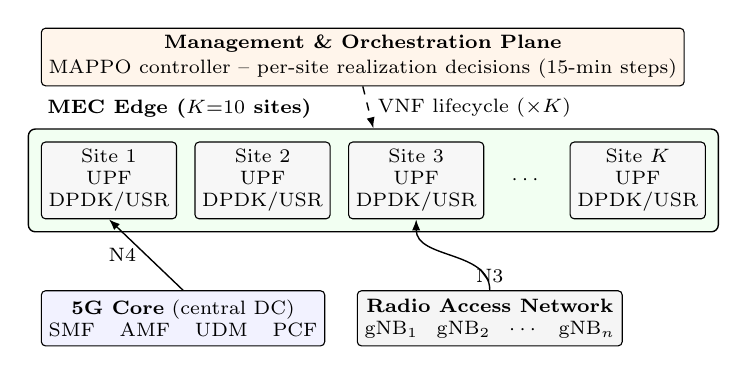
\begin{tikzpicture}[node distance=2.2mm]
% MANO plane
\node[blk,fill=orange!8,minimum width=68mm] (mano)
  {\textbf{Management \& Orchestration Plane}\\[1pt]
   \scriptsize MAPPO controller -- per-site realization decisions (15-min steps)};
% MEC sites
\node[blk,below=7mm of mano.south west,anchor=north west,minimum width=14mm] (s1)
  {Site 1\\\scriptsize UPF\\\scriptsize DPDK/USR};
\node[blk,right=of s1,minimum width=14mm] (s2) {Site 2\\\scriptsize UPF\\\scriptsize DPDK/USR};
\node[blk,right=of s2,minimum width=14mm] (s3) {Site 3\\\scriptsize UPF\\\scriptsize DPDK/USR};
\node[right=of s3,font=\scriptsize] (dots) {$\cdots$};
\node[blk,right=of dots,minimum width=14mm] (sk) {Site $K$\\\scriptsize UPF\\\scriptsize DPDK/USR};
\begin{scope}[on background layer]
\node[grp,fill=green!5,fit=(s1)(sk),label={[font=\scriptsize\bfseries]above left:MEC Edge ($K{=}10$ sites)}] (mec) {};
\end{scope}
% core + ran
\node[blk,fill=blue!5,below=9mm of s1.south west,anchor=north west,minimum width=34mm] (core)
  {\textbf{5G Core} (central DC)\\\scriptsize SMF \;\, AMF \;\, UDM \;\, PCF};
\node[blk,fill=gray!8,right=4mm of core,minimum width=30mm] (ran)
  {\textbf{Radio Access Network}\\\scriptsize gNB$_1$ \, gNB$_2$ \, $\cdots$ \, gNB$_n$};
% flows
\draw[fl,dashed] (mano.south) -- ($(mec.north)+(0,0.0)$)
  node[midway,right,font=\scriptsize] {VNF lifecycle ($\times K$)};
\draw[fl] (core.north) -- (s1.south) node[midway,left,font=\scriptsize] {N4};
\draw[fl] (ran.north) to[out=90,in=-90] (s3.south);
\node[font=\scriptsize] at ($(ran.north)+(0.0,0.18)$) {N3};
\end{tikzpicture}}
\caption{5G deployment model. The MAPPO controller operates at the
management and orchestration plane and issues container start/stop
operations to switch each MEC site between DPDK and USR realizations. The
5G Core control plane stays centralised, and the SMF continues to issue
N4/PFCP session rules to the active UPF at each site.}
\label{fig:deploy}
\end{figure}

% ===========================================================================
\section{Multi-Site Control Problem}
\label{sec:problem}
% ===========================================================================
\subsection{Per-site observation and objective}
Each agent observes a 14-dimensional state at step $t$, formed by the
current load $\lambda_{i,t}$, an 8-step history window
$\lambda_{i,t-1},\dots,\lambda_{i,t-8}$, the one-step forecast
$\hat{\lambda}_{i,t+1}$, the previous action $a_{i,t-1}$, the previous
QoS score $Q_{i,t-1}$, the previous specific energy
$\SECt_{i,t-1}$, and a normalised cooldown-progress signal. The
cooperative objective is the discounted sum of per-cluster rewards over
an episode of length $T\,{=}\,1009$,
\begin{equation}
J(\pi) = \mathbb{E}_{\pi}\!\left[\sum_{t=0}^{T-1}\gamma^{t}\sum_{i=1}^{K}r_{i,t}\right],
\qquad \gamma = 0.995 .
\end{equation}
Coupling across agents enters only through the joint cumulative reward.
Per-cluster dynamics are independent given the realization choice, and we
defer shared-resource extensions such as a common CPU pool to future
work.

\subsection{Physics-grounded reward}
Following the single-site formulation of~\cite{ref:comcom} but removing
its parallel flat switching constant, the per-step reward is
\begin{equation}
\label{eq:reward}
r_{i,t} = -\bigl(\alpha\,\SECt_{i,t}
            + \lambda_{\mathrm{QoS}}\max(0,\tau-Q_{i,t})
            + L^{\mathrm{CD}}_{i,t}\bigr).
\end{equation}
The specific energy term now carries both steady-state and transition
power. With the twin's per-transition spike energy
$E^{\mathrm{sw}}_{i,t}\,{=}\,P_{\mathrm{new}}(\lambda_{i,t})\,
t^{\mathrm{act}}_{\mathrm{new}}$ and a step duration
$\Delta t\,{=}\,900$\,s, we define
\begin{align}
P^{\mathrm{eff}}_{i,t} &= P^{\mathrm{steady}}_{i,t} + E^{\mathrm{sw}}_{i,t}/\Delta t,\\
\SECt_{i,t} &= P^{\mathrm{eff}}_{i,t}\,/\,\max(\lambda_{i,t},\varepsilon)\quad[\text{W/Mbps}].
\end{align}
The QoS score $Q_{i,t}\,{=}\,\min(\mathrm{score}_{d}(d_{i,t}),
\mathrm{score}_{\ell}(\ell_{i,t}))\,{\in}\,[0,1]$ grades delay and loss
against their budgets, and $L^{\mathrm{CD}}_{i,t}$ is a soft
anti-oscillation penalty that fires when a switch happens inside a
cooldown window. The constants are
$(\alpha,\lambda_{\mathrm{QoS}},\tau)\,{=}\,(100,30,0.9)$, with cooldown
period 4 steps and cost $c_{\mathrm{CD}}\,{=}\,0.5$, matching the
paper-aligned values of~\cite{ref:comcom}. The asymmetry between DPDK and
USR switching costs now emerges automatically from
$t^{\mathrm{act}}_{\mathrm{DPDK}}\,{\gg}\,t^{\mathrm{act}}_{\mathrm{USR}}$
and from load scaling, since a DPDK activation under heavy traffic costs
more than one under light traffic, as it physically should. A previous
revision used flat per-event constants running in parallel to the twin's
$E^{\mathrm{sw}}$, and we removed that redundancy.

\subsection{Classical baseline derivation}
The threshold and hysteresis baselines use operating points derived from
the twin rather than hand-tuned. Sweeping the twin gives an energy
break-even at 91.0~Mbps, where USR power first exceeds DPDK power, and a
QoS limit at 149.0~Mbps, the last load where USR stays safe. Taking the
minimum and subtracting a 10~Mbps safety margin yields a decision
threshold of 81.0~Mbps. A paper-faithful hysteresis band set to twice the
forecaster MAE is 221.3~Mbps, which is more than $2.7\times$ the decision
threshold. As a result the lower threshold collapses to zero and the
auto-tuned hysteresis controller never leaves DPDK after the first step.
This is the honest behaviour of naive hysteresis at this forecaster
accuracy, not a bug. To give the classical family its strongest possible
form, we additionally sweep a narrower band over
$\{5,10,20,50,100\}$~Mbps and report the best operating point
(Section~\ref{sec:results}).

% ===========================================================================
\section{Cooperative MARL Controllers}
\label{sec:method}
% ===========================================================================
\noindent\textbf{MAPPO (proposed).} MAPPO~\cite{ref:mappo} uses a
parameter-shared actor, an MLP $14\,{\to}\,64\,{\to}\,64\,{\to}\,2$ with
5{,}250 parameters in which one network handles every agent's per-step
decision, together with a centralised critic on the global state, an MLP
$140\,{\to}\,128\,{\to}\,128\,{\to}\,K$ with 35{,}850 parameters. The
global state is the concatenation of all per-agent observations
($K\,{\times}\,14\,{=}\,140$). Training uses PPO
clipping~\cite{ref:ppo} on per-agent ratios with
GAE~\cite{ref:gae} ($\lambda\,{=}\,0.9$), per-agent advantage
normalisation over $(T,K)$ to absorb the cross-cluster reward-scale
differences, and reward scaling of $0.01$ to balance actor and critic
losses. We run 200k environment steps with $n_{\mathrm{steps}}\,{=}\,1024$,
$n_{\mathrm{epochs}}\,{=}\,10$, minibatch 256, learning rate
$3\,{\times}\,10^{-4}$, and entropy coefficient $0.05$.
Best-of-validation checkpoint selection is load-bearing, because without
it a late-stage policy collapse on a near-zero-load step produces an
unusable final-step model.

\noindent\textbf{IPPO ensemble (ablation).} The IPPO ensemble trains
$K\,{=}\,10$ independent Stable-Baselines3~\cite{ref:sb3} PPO actors, one
per cluster, on each cluster's 14-dimensional observation with identical
hyperparameters. At evaluation the per-cluster policies are stacked. By
construction the ensemble consumes $K$ times the training budget, which
is its nominal compute advantage over the shared-actor design.

\noindent\textbf{Centralised PPO (ablation).} The centralised baseline is
a single SB3 PPO on the joint 140-dimensional observation with a
$\mathrm{MultiDiscrete}([2]^{K})$ joint action, otherwise matched in
reward, budget, and checkpoint selection.

\noindent\textbf{Evaluation protocol.} Each trained controller is
evaluated once on the test slice with a deterministic policy and a fixed
environment seed for reset, over the full 1009-step episode on every
cluster. MAPPO and IPPO are run at eight seeds
$\{1,7,13,23,42,64,77,99\}$, and centralised PPO at four seeds, since its
failure mode is unambiguous at any sample size. Classical baselines are
deterministic. We report reward as the unweighted sum over clusters and
steps, total fleet energy in watt-hours, the QoS-violation rate (the
fraction of cluster-steps whose delay or loss budget is exceeded), the
USR usage share, and the switch count.

% ===========================================================================
\section{Results}
\label{sec:results}
% ===========================================================================
\subsection{Headline comparison}
Table~\ref{tab:headline} reports test-slice means across all controllers.
MAPPO attains the lowest reward magnitude, the lowest energy, and the
lowest QoS-violation rate among the trained policies. On reward it
improves on the swept-best classical baseline (hysteresis at band
50~Mbps) by 10.0\%, on always-DPDK by 21.8\%, and on the centralised PPO
by 61.0\%, which is the 10 to 61\% range quoted in the abstract. The
margin over the IPPO ensemble is much smaller in magnitude (154 reward
units, about 2.7\%) but is statistically robust, as the next subsection
shows. MAPPO is also the lowest-energy trained controller at 1967~Wh,
ahead of IPPO at 1973~Wh and well ahead of always-DPDK at 2071~Wh. The
energy gap to IPPO is small, so the reward advantage comes less from raw
watt-hours and more from better-placed USR usage that avoids QoS
penalties (Section~\ref{sec:results}-C).

\begin{table}[!t]
\centering
\caption{Test-slice comparison ($K\,{=}\,10$, 1009-step episode). MAPPO
and IPPO at 8 seeds, centralised PPO at 4. Reward is the unweighted sum
over clusters and steps; QoSv is the QoS-violation rate.}
\label{tab:headline}
\renewcommand{\arraystretch}{1.12}
\setlength{\tabcolsep}{3.2pt}
\footnotesize
\begin{tabular}{@{}lr@{\;}crrr@{}}
\toprule
Controller & Reward & $n$ & Wh & QoSv\% & USR\% \\
\midrule
\textbf{MAPPO (ours)}      & $\mathbf{-5633\!\pm\!100}$ & 8 & $\mathbf{1967}$ & $\mathbf{0.52}$ & 7.8 \\
IPPO ensemble              & $-5787\!\pm\!89$           & 8 & 1973            & 0.57           & 8.1 \\
Hysteresis ($b{=}50$)      & $-6262$                    & -- & 1995           & 0.68           & 7.5 \\
Hysteresis ($b{=}20$)      & $-6543$                    & -- & 1971           & 0.94           & 11.5 \\
Always-DPDK                & $-7201$                    & -- & 2071           & 0.38           & 0.0 \\
Threshold (81\,Mbps)       & $-7623$                    & -- & 1970           & 1.42           & 14.0 \\
Centralised PPO            & $-14{,}458\!\pm\!4509$     & 4 & 2130            & 3.73           & 9.3 \\
\bottomrule
\end{tabular}
\end{table}

\subsection{Statistical significance}
A paired bootstrap over the eight seed-matched MAPPO minus IPPO deltas
(10{,}000 resamples) places the architectural gap at $+154$ reward units,
with a 95\% CI of $[+28,+262]$ and a one-sided $p\,{=}\,0.009$. The
interval excludes zero by a clear margin, so the MAPPO win over IPPO is
significant at the 0.01 level under the physics-grounded reward.
Fig.~\ref{fig:bootstrap}(a) shows that seven of the eight seeds favour
MAPPO. The single counter-example is seed 13, where MAPPO converged to a
slightly more aggressive USR policy (0.67\% QoS violation, 364 switches,
against the MAPPO averages of 0.52\% and 297) and IPPO happened to train
its single best ensemble of the set. Fig.~\ref{fig:bootstrap}(b) shows
the bootstrap distribution. Both architectures have comparable
seed-to-seed reward range (MAPPO 315, IPPO 243), so MAPPO is slightly
less stable across seeds but reliably better on the mean.

\begin{figure}[!t]
\centering
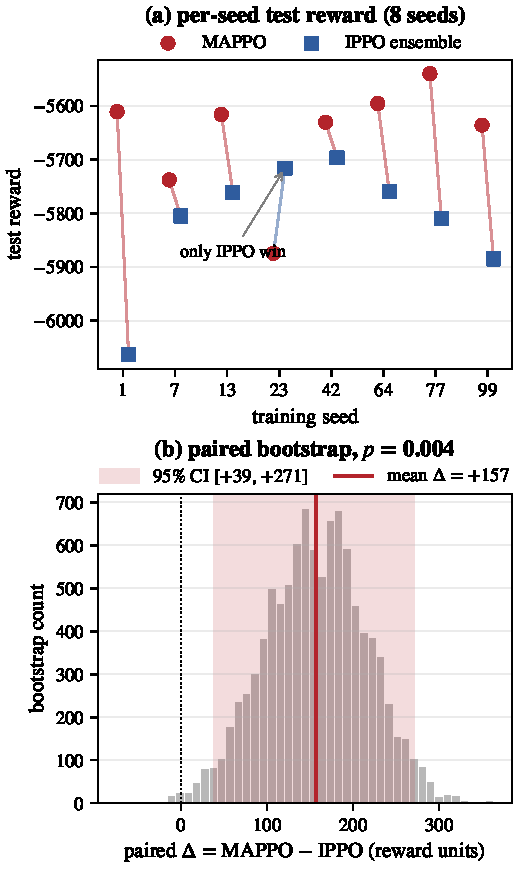
\includegraphics[width=\columnwidth]{figures/fig_bootstrap.pdf}
\caption{(a) Per-seed test reward for MAPPO (circles) and the IPPO
ensemble (squares) over eight seeds, with paired lines connecting
seed-matched runs. Seed 13 is the only seed where IPPO wins. (b)
Paired-bootstrap distribution (10{,}000 resamples) of the mean
$\Delta\,{=}\,\mathrm{MAPPO}-\mathrm{IPPO}$ delta, with the 95\% CI
$[+28,+262]$ excluding zero ($p\,{=}\,0.009$).}
\label{fig:bootstrap}
\end{figure}

\subsection{Cross-cluster transfer}
Fig.~\ref{fig:percluster} breaks the test reward down by cluster, with
clusters sorted by mean offered load. MAPPO wins on 7 of 10 clusters,
ties on the high-load DPDK-bound cluster c3, and loses by a small margin
on two mid-load clusters (c2 by 8.8\% and c8 by 0.4\%). The clearest wins
are on the low- and mid-load clusters, c5 ($+8.6\%$), c0 ($+6.6\%$), c7
($+4.3\%$), and c4 ($+3.4\%$), which are exactly the sites where USR is
the right call but a per-cluster IPPO has limited sample signal to find
it. On c0, the lowest-load cluster, MAPPO's shared actor drives the most
USR usage and the largest gap to always-DPDK. The shared actor, trained
simultaneously on the data-rich low-load clusters, transfers the
``USR-at-low-predicted-load'' rule to sites where an independent learner
would stay close to DPDK. The small regression on c2 is the cost of
policy sharing on a heterogeneous fleet, where MAPPO occasionally tries
USR on a cluster that an independent learner has correctly fixed to DPDK,
and it is more than offset by the low-load wins. On the highest-load
cluster c9, with peaks near 5.8~Gbps, a few IPPO seeds tried USR and were
punished, leaving the IPPO mean slightly below always-DPDK, whereas MAPPO
correctly stays on DPDK across all eight seeds.

\begin{figure*}[!t]
\centering
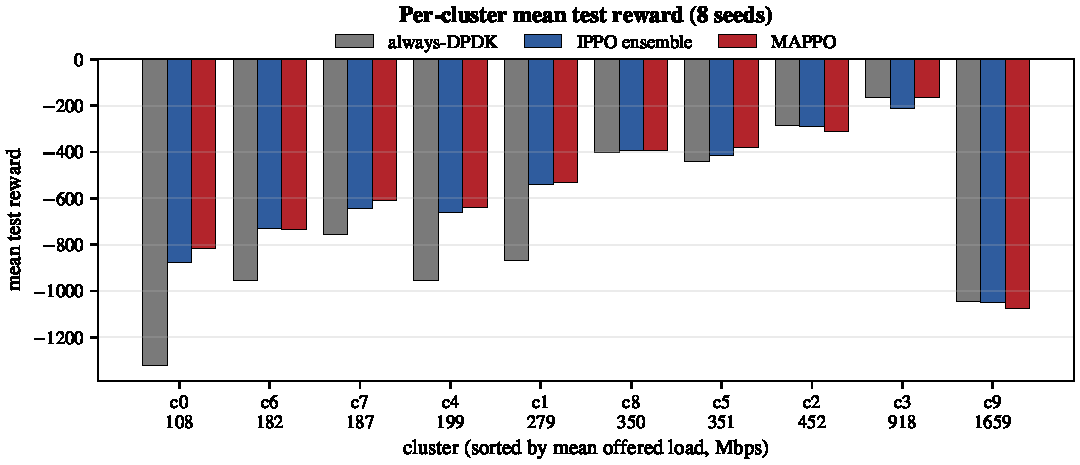
\includegraphics[width=\textwidth]{figures/fig_per_cluster.pdf}
\caption{Per-cluster mean test reward (8 seeds) for always-DPDK, the IPPO
ensemble, and MAPPO, with clusters sorted by mean offered load (Mbps).
MAPPO's advantage concentrates on the low- and mid-load clusters, where
independent learning lacks the signal to leave DPDK. The high-load
clusters c3 and c9 are DPDK-bound for every controller.}
\label{fig:percluster}
\end{figure*}

\subsection{Classical-baseline sensitivity}
Table~\ref{tab:hyst} sweeps the hysteresis band over five widths, with
$t_{up}$ fixed at the derived 81~Mbps decision point and a one-step
cooldown. Two facts stand out. First, the hand-picked 20~Mbps band used
in earlier iterations is not the best classical operating point. Widening
to 50~Mbps cuts switching from 215 to 111 events and improves reward by
281 units, while a band of 100~Mbps drives $t_{down}$ to zero and
collapses the controller to always-DPDK. Second, no setting of the band
closes the gap to MAPPO. Even at the sweep optimum, hysteresis is 629
reward units behind MAPPO, far outside the MAPPO minus IPPO 95\% CI and
any per-seed range. The classical controller's fundamental limit at this
forecaster accuracy is that any band wide enough to suppress
noise-induced switching either degenerates to always-DPDK or admits a
non-trivial QoS-violation rate.

\begin{table}[!t]
\centering
\caption{Hysteresis band sweep ($t_{up}\,{=}\,81$~Mbps, cooldown 1 step).
Band 50~Mbps is the strongest classical operating point, still 629 reward
units behind MAPPO.}
\label{tab:hyst}
\renewcommand{\arraystretch}{1.12}
\setlength{\tabcolsep}{4.5pt}
\footnotesize
\begin{tabular}{@{}rrrrrl@{}}
\toprule
Band & $t_{down}$ & Reward & Switches & QoSv\% & Regime \\
\midrule
5   & 76 & $-7047$ & 317 & 1.16 & over-switching \\
10  & 71 & $-6923$ & 285 & 1.11 & over-switching \\
20  & 61 & $-6543$ & 215 & 0.94 & prior hand-pick \\
\textbf{50}  & \textbf{31} & $\mathbf{-6262}$ & \textbf{111} & \textbf{0.68} & \textbf{best classical} \\
100 & 0  & $-7201$ & 0   & 0.38 & collapses to DPDK \\
\bottomrule
\end{tabular}
\end{table}

A complementary cooldown sweep on MAPPO (seed 42) around the default
period 4 and cost 0.5 confirms the headline does not hinge on these
hyperparameters. Lowering the cost to 0.1 lets the controller switch 58\%
more often and costs 526 reward units, while raising it to 1.0
overpenalises switching and costs 264 units. Varying the period between 2
and 6 steps moves reward by at most 144 units. The default sits in the
centre of a soft plateau whose width is on the order of the MAPPO minus
IPPO gap and well inside the gap to the strongest classical baseline.

\subsection{Why centralised PPO fails}
The centralised single-MLP PPO sees the same problem, reward, and
training budget, yet it trails MAPPO by 61\% with a seed-to-seed range of
about 9{,}930 reward units (per-seed rewards $-11{,}202$, $-12{,}718$,
$-12{,}779$, $-21{,}132$). Its energy at 2130~Wh is worse than
always-DPDK, because it spends transition energy without the offsetting
low-load USR benefit. Inspecting per-cluster behaviour reveals the
failure mode. The joint factored softmax collapses one or two clusters to
mostly-USR even when their load is unsafe for it, for example one seed
drives cluster c6 to 98\% USR with a 46\% QoS-violation rate, and another
drives c7 to 56\% USR with a 23\% violation rate. A single unsafe cluster
of this kind dominates the joint reward and never recovers, because the
$140$-dimensional to $10$-dimensional factored softmax cannot factor the
per-cluster substructure within the training budget. The diagnosis is
architectural rather than optimisational. Ten parameter-sharing
$14$-to-$2$ policies are a much easier optimisation than one joint policy
over a $2^{K}$ action space.

% ===========================================================================
\section{Conclusion}
\label{sec:conclusion}
% ===========================================================================
We cast per-site DPDK/USR realization switching across $K\,{=}\,10$
heterogeneous MEC clusters as a cooperative MARL problem on a
measurement-grounded digital twin, under a physics-grounded reward that
folds the twin's measured switching energy into specific energy
consumption. On a 10.5-day held-out test slice, MAPPO with a
shared-parameter actor and a centralised critic beats an IPPO ensemble,
a centralised single-MLP PPO, and the swept-best classical hysteresis
controller by 10 to 61\% on reward. The win over IPPO is small in
magnitude but statistically significant (paired bootstrap
$p\,{=}\,0.009$, 95\% CI $[+28,+262]$), and it concentrates on the
data-poor low-load clusters, which is consistent with cross-cluster
policy transfer through the shared actor. The practical message is that
for energy-aware UPF coordination at the edge, the choice of coordination
architecture matters more than the choice of algorithm. Future work will
hold out clusters at training time to test zero-shot transfer directly,
add shared-resource coupling such as a common CPU pool, and validate the
twin against a live DPDK/USR testbed.

% ---------------------------------------------------------------------------
\begin{thebibliography}{99}
\footnotesize

\bibitem{ref:carbon}
Y.~Ding, H.~Duan, M.~Xie, J.~Rao, J.~J.~Wang, and W.~Zhang, ``Carbon
emissions and mitigation potentials of 5G base stations in China,''
\emph{Resources, Conservation and Recycling}, vol.~182, p.~106330, 2022.

\bibitem{ref:rischke}
J.~Rischke, C.~Vielhaus, P.~Sossalla, J.~Wang, and F.~H.~P.~Fitzek,
``Comparison of UPF acceleration technologies and their tail-latency for
URLLC,'' in \emph{Proc.\ IEEE NFV-SDN}, 2022, pp.~146--151.

\bibitem{ref:slices}
S.~Afshar Borji, R.~Bruschi, C.~E.~Costa, and C.~Lombardo, ``Dynamic
energy-efficient User Plane Function selection in 5G networks,'' in
\emph{Proc.\ IFIP SLICES Workshop}, 2025.

\bibitem{ref:comcom}
S.~Afshar Borji, R.~Bruschi, C.~Lombardo, R.~Bolla, and C.~E.~Costa,
``AI-driven energy-efficient orchestration of User Plane Functions in 5G
Core networks,'' \emph{Computer Communications}, 2026, under review,
manuscript COMCOM-S-26-00430.

\bibitem{ref:mappo}
C.~Yu, A.~Velu, E.~Vinitsky, J.~Gao, Y.~Wang, A.~Bayen, and Y.~Wu, ``The
surprising effectiveness of PPO in cooperative multi-agent games,'' in
\emph{Adv.\ Neural Inf.\ Process.\ Syst.\ (NeurIPS)}, vol.~35, 2022.

\bibitem{ref:sb3}
A.~Raffin, A.~Hill, A.~Gleave, A.~Kanervisto, M.~Ernestus, and
N.~Dormann, ``Stable-Baselines3: Reliable reinforcement learning
implementations,'' \emph{J.\ Mach.\ Learn.\ Res.}, vol.~22, no.~268,
pp.~1--8, 2021.

\bibitem{ref:leyva}
I.~Leyva-Pupo and C.~Cervell\'o-Pastor, ``Efficient solutions to the
placement and chaining problem of User Plane Functions in 5G,''
\emph{J.\ Netw.\ Comput.\ Appl.}, vol.~197, p.~103253, 2022.

\bibitem{ref:bellin}
A.~Bellin, N.~Di Cicco, D.~Munaretto, and F.~Granelli, ``Power
consumption-aware 5G edge UPF selection using deep reinforcement
learning,'' in \emph{Proc.\ IEEE NFV-SDN}, 2024, pp.~1--6.

\bibitem{ref:zhu}
Y.~Zhu et al., ``Multi-agent deep reinforcement learning for
UAV-assisted 5G network slicing: A comparative study of MAPPO, MADDPG,
and MADQN,'' \emph{arXiv preprint arXiv:2512.03835}, 2024.

\bibitem{ref:qmix}
T.~Rashid, M.~Samvelyan, C.~Schroeder de Witt, G.~Farquhar, J.~Foerster,
and S.~Whiteson, ``QMIX: Monotonic value function factorisation for deep
multi-agent reinforcement learning,'' in \emph{Proc.\ Int.\ Conf.\ Mach.\
Learn.\ (ICML)}, 2018.

\bibitem{ref:vdn}
P.~Sunehag et al., ``Value-decomposition networks for cooperative
multi-agent learning based on team reward,'' in \emph{Proc.\ Int.\ Conf.\
Auton.\ Agents Multi-Agent Syst.\ (AAMAS)}, 2018.

\bibitem{ref:ppo}
J.~Schulman, F.~Wolski, P.~Dhariwal, A.~Radford, and O.~Klimov,
``Proximal policy optimization algorithms,'' \emph{arXiv preprint
arXiv:1707.06347}, 2017.

\bibitem{ref:gae}
J.~Schulman, P.~Moritz, S.~Levine, M.~Jordan, and P.~Abbeel,
``High-dimensional continuous control using generalized advantage
estimation,'' in \emph{Proc.\ Int.\ Conf.\ Learn.\ Represent.\ (ICLR)},
2016.

\bibitem{ref:ndt}
P.~Almasan, M.~Ferriol-Galm\'es, J.~Paillisse et al., ``Network digital
twin: Context, enabling technologies, and opportunities,'' \emph{IEEE
Communications Magazine}, vol.~60, no.~11, pp.~22--27, 2022.

\bibitem{ref:rapl}
K.~N.~Khan, M.~Hirki, T.~Niemi, J.~K.~Nurminen, and Z.~Ou, ``RAPL in
action: Experiences in using RAPL for power measurements,'' \emph{ACM
Trans.\ Model.\ Perform.\ Eval.\ Comput.\ Syst.}, vol.~3, no.~2, 2018.

\bibitem{ref:pz}
J.~K.~Terry et al., ``PettingZoo: Gym for multi-agent reinforcement
learning,'' \emph{arXiv preprint arXiv:2009.14471}, 2021.

\end{thebibliography}

\end{document}
